\section{Esolangs (Linguagens exóticas)}

\begin{frame}[fragile]{Benfuge (não use)}
\small{Benfuge é uma linguagem escrita bidimensionalmente, seu código pode andar em 4 direções.}
\lstset{language=Rust, style=boxed}
\begin{lstlisting}
>                v
v ,,,,,"Hello"<
>48*,           v
v,,,,,,"World!"<
>25*,@
\end{lstlisting}
\small{https://catseye.tc/article/Languages.md\#befunge-93}
\end{frame}

\begin{frame}[fragile]{Whitespace (não use)}
\begin{figure}[ht!]
  \centering
  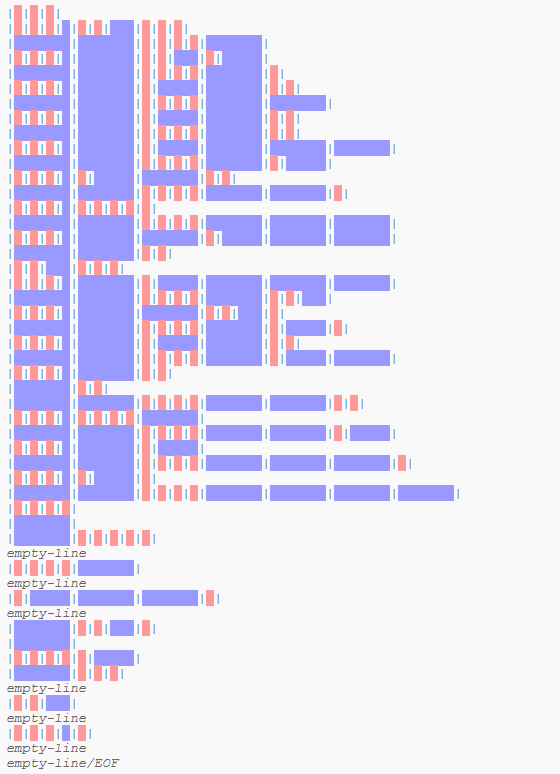
\includegraphics[scale=0.4]{images/whitespace.png}
\end{figure}
\end{frame}

\begin{frame}[fragile]{BIRL (Bambam's "It's show time" Recursive Language)}
\begin{figure}[ht!]
  \centering
  
\includegraphics[scale=0.1]{images/birl.png}
\end{figure}
\lstset{language=Rust, style=boxed}
\begin{lstlisting}
HORA DO SHOW
    CE QUER VER ESSA PORRA? ("Hello, World!\n");
    BORA CUMPADE 0;
BIRL
\end{lstlisting}
\small{Baseada em ArnoldC segundo o autor ``Deve ser utilizada apenas por quem realmente constrói fibra e não é água com código.'' (Made in Brazil)}
\small{https://birl-language.github.io/ }
\end{frame}
